\documentclass[a4paper,12pt]{article}
\usepackage{amsmath}
\usepackage{amsfonts}
\usepackage{amssymb}
\pagestyle{headings}
\title{Wiederholung für das Abitur im Fach Mathematik}
\date{}
\begin{document}
\maketitle
\tableofcontents

\section{Kurvendiskussion}
	\subsection{Übersicht}
		\begin{enumerate}
			\item Definitionsbereich:
			\item Symetrie:
				\begin{enumerate}
					\item Achsensymetrie: $f(x)=f(-x)$
					\item Punktsymetrie: $f(-x) = -f(x)$
				\end{enumerate}
			\item Achsenschnittpunkt:
				\begin{enumerate}
					\item y-Achse: $f(0)$
					\item x-Achse/Nullstellen: $f(x)=0$
				\end{enumerate}
			\item Extrempunkte:
				\begin{enumerate}
					\item Notwendige Bedingung: $f^{\prime}(x)=0$
					\item Hinreichende Bedingung: $f^{\prime}(x)=0 \ \& f^{\prime\prime}(x) \neq0$
					\item Hochpunkt: $f^{\prime\prime}(x) < 0$
					\item Tiefpunkt: $f^{\prime\prime}(x)>0$
				\end{enumerate}
			\item Wendepunkte:
				\begin{enumerate}
					\item Notwendige Bedingung: $f^{\prime\prime}(x)=0$
					\item Hinreichende Bedingung: $f^{\prime\prime}(x)=0 \ \& f^{\prime\prime\prime}(x) \neq0$
					\item Links-Rechts-Wendepunkt: $f^{\prime\prime\prime}(x) < 0$
					\item Rechts-Links-Wendepunkt: $f^{\prime\prime\prime}(x)>0$
				\end{enumerate}
			\item Sattelpunkt:
				\begin{enumerate}
					\item Notwendige Bedingung: $f^{\prime}(x)=0$
					\item Hinreichende Bedingung: $f^{\prime\prime}(x)=0$
				\end{enumerate}
		\end{enumerate}
	\subsection{Nullstellen}
		\subsubsection{PQ-Formel}
			$$
x_{1, 2} = - \frac{P}{2} \pm \sqrt{\frac{p^{2}}{4}-4}
			$$
		\subsubsection{Quadratische Ergänzung}
			binomische Formeln:
				\begin{enumerate}
					\item $(a+b)^{2} = 2a^{2}+2ab+b^{2}$
					\item $(a-b)^{2} = 2a^{2}-2ab+b^{2}$
					\item $(a+b)^{2}*(a-b)^{2}  = a^{2}-b^{2}$
				\end{enumerate}
		\subsubsection{Wendepunkte}
			\begin{enumerate}
				\item Notwendige Bedingung: $f^{\prime\prime}(x)=0$
				\item Hinreichende Bedingung: $f^{\prime\prime\prime}(x)=+\neq0 \rightarrow rechts-links-Wendepunkt´$
				\item Einsetzen in f(x): $f(x)=a$
			\end{enumerate}
\section{Vektoren}
	\subsection{Skalarprodukt}
		Mithilfe des Skalarprodukts kann man überprüfen ob zwei Vektoren orthogonal (d.h. in einem 90° Winkel) zueinander sind.	Die allgemeine Formel lautet:
		$$
		\vec{AB} \cdot \vec{AC} = 
		\begin{pmatrix} 
			x_{1} \\
			x_{2} \\
			x_{3} 
		\end{pmatrix}
		\cdot 
		\begin{pmatrix} 
			y_{1} \\
			y_{2} \\
			y_{3}
		\end{pmatrix} = x_{1} \cdot y_{1}+x_{2} \cdot y_{2}+x_{3} \cdot y_{3}
		$$
		Wenn das Skalarprodukt:
			\begin{itemize}
				\item $=0 \text{ ist} \rightarrow \text{Die Vektoren liegen } \textbf{orthogonal } \text{zueinander/90°}$
				\item $\neq 0 \text{ist} \rightarrow \text{Die Vektoren liegen } \textbf{nicht } \text{orthogonal zueinander}$
			\end{itemize}
	\subsection{Lage zweier Geraden zueinander bestimmen}
	\subsection{Mittelpunkt einer Geraden bestimmen}
		$$
\vec{m} = \frac{1}{2}*(\vec{b}+\vec{c})=\frac{1}{2}*
\begin{pmatrix}
\begin{pmatrix} 
x_{1}+y_{1} \\
x_{2}+y_{2} \\
x_{3}+y_{3}
\end{pmatrix}
\end{pmatrix}
$$
	\subsection{Längenformel eines Vektors}
		$$
\sqrt{a^{2}+b^{2}+c^{2}}
$$
		\textbf{Beispiel:}
		$$
\sqrt{2^{2}+2^{2}+(-1)^{2}}=
\sqrt{4+4+1}=
\sqrt{9}=3
$$
	\subsection{Punktprobe}
		$$
\begin{pmatrix} 
a_{1} \\
a_{2} \\
a_{3}
\end{pmatrix}+k*
\begin{pmatrix} 
b_{1} \\
b_{2} \\
b_{3}
\end{pmatrix}=
\begin{pmatrix} 
c_{1} \\
c_{2} \\
c_{3}
\end{pmatrix} \rightarrow
\begin{vmatrix}
a_{1}+b_{1}*k=c_{1} \\
a_{2}+b_{1}*k=c_{2} \\
a_{3}+b_{1}*k=c_{3}
\end{vmatrix} \rightarrow
\begin{vmatrix}
k=x \\
k=y \\
k=z
\end{vmatrix}
$$
		\textbf{Beispiel:}
			$$
\begin{pmatrix} 
-2 \\
3 \\
1
\end{pmatrix}+k*
\begin{pmatrix} 
2 \\
-5 \\
7
\end{pmatrix}=
\begin{pmatrix} 
-12 \\
23 \\
-34
\end{pmatrix} \rightarrow
\begin{vmatrix}
-2+2*k=-12\\
3-5*k=23\\
1+7*k=-34
\end{vmatrix} \rightarrow
\begin{vmatrix}
k=-5 \\
k=-4 \\
k=-5 \\
\end{vmatrix}
$$
\section{Stochastik}
	\subsection{Empirische Standardabweichung}
		$$ \overline{s} = \sqrt{p_{1} \cdot (x_{1}-\overline{x})^{2}+p_{2} \cdot (x_{2}-\overline{x})^{2}+p_{3} \cdot (x-\overline{x})^{3}+...} $$
	\subsection{Erwartungswert}
		$$ E(x) = 1 \cdot P(X = 1) + 2 \cdot P(X = 2) + 3 \cdot P(X = 3) + ... $$
	\subsection{Binomialkoeffizient}
$$
\binom{n}{k} =  \frac{n!}{k!\,(n-k)!}
$$

$$
\text{binomPDF: } P(X=Y) = \binom{n}{k} \cdot p^{k} \cdot (1-p)^{n-k}
$$

$$
\text{binomCDF: } P(X\leq Y) = p(x=y) + p(x=y-1) + ... + p(x=y-y)
$$
	\subsection{Vier-Felder-Tafel}
	\begin{center}
	\begin{tabular}{|c|c|c|c|}
	\hline 
	 & $B$ & $\overline{B}$ &  \\ 
	\hline
	$A$ & Wahrscheinlichkeit $AB$ & Wahrscheinlichkeit $A\overline{B}$ & Wahrscheinlichkeit $A$ \\ 
	\hline
	$\overline{A}$ & Wahrscheinlichkeit $\overline{A}B$ & Wahrscheinlichkeit $\overline{AB}$ & Wahrscheinlichkeit $\overline{A}$ \\ 
	\hline
	 & Wahrscheinlichkeit $B$ & Wahrscheinlichkeit $\overline{B}$ & $1$ \\ 
	\hline 
	\end{tabular} 
	\end{center}
	\textbf{Beispiel:} \\
	\\
	\begin{tabular}{|c|c|c|c|}
	\hline 
	 & $B$ & $\overline{B}$ &  \\ 
	\hline
	$A$ & $0.21$ & $0.49$ & $0.7$ \\ 
	\hline
	$\overline{A}$ & $0.06$ & $0.24$ & $0.3$ \\ 
	\hline
	 & $0.27$ & $0.73$ & $1$ \\ 
	\hline 
	\end{tabular}
	\subsection{Sigma-Regeln}
	\subsubsection{Intervalle abschätzen für sigma}
	\begin{center}
	$90\% \rightarrow 1.64 \cdot \sigma$ \\
	$95\% \rightarrow 1.96 \cdot \sigma$ \\
	$99\% \rightarrow 2.58 \cdot \sigma$
	\end{center}
	
	\subsection{Erwartungswert}
	$$ \mu = n \cdot p $$
	\subsection{Standardabweichung}
	$$ \sigma = \sqrt{n \cdot p \cdot (1-p)} $$
	\subsection{Sigma-Regeln andwenden für }
		\begin{enumerate}
			\item Gegeben: n, p
			\item $ \mu = n \cdot p$
			\item $\sigma = \sqrt{n \cdot p \cdot (1-p)}$ $\rightarrow$ Wenn $\sigma >$ 3 ist:
			\begin{enumerate}
				\item $1.64 \cdot \sigma = d$
				\item $\mu -d \leq X \leq \mu + d$
				\item $P(\mu + d (aufrunden) < X <\mu + d (abrunden))$
				\item $P(\mu + d (abrunden) < X <\mu + d (aufrunden))$
				\item Hinweis: Dies kann mit dem binomCDF befehl des CAS berechnet berechnet werden.
				\item Das Ergebnis welches am nächsten über 0.9 liegt ist das bessere Ergebnis
			\end{enumerate}
		\end{enumerate}
	\textbf{Beispiel:}
	\begin{enumerate}
			\item Gegeben: $n = 920$,  $p = 58$
			\item $ \mu = 920 \cdot 0.58 = 533.6$
			\item $\sigma = \sqrt{920 \cdot 0.58 \cdot (0.42)} = 14.9703$ $\rightarrow$ Wenn $\sigma$ > 3 ist:
			\begin{enumerate}
				\item $1.64 \cdot 14.9703 = 24.5513$
				\item $533.6 - 24.5513 \leq X \leq 533.5 + 24.5513 \rightarrow 509.0487 \leq X \leq 558.1513$
				\item $P(510 < X < 558) = 0.8982$
				\item $P(509 < X <559) = 0.9114$
				\item $\rightarrow$ Das richtige Ergebnis ist $P(509 \leq X \leq 559)$
			\end{enumerate}
		\end{enumerate}
	\subsection{Histogramme}
	Histogramme stellen die Wahrscheinlichkeit einer Anzahl von Treffern graphisch dar. Sie sehen Glockenförmig aus wobei die Spitze den Erwartungswert darstellt, welcher die größte Wahrscheinlichkeit besitzt. Die y-Achse gibt die Wahrscheinlichkeit an, während die x-Achse die Anzahl der Ereignisse bzw. Treffer angibt.
	\subsubsection{Beispiel}
	\begin{itemize}
		\item n = 15
		\item p = 0.38
	\end{itemize}
	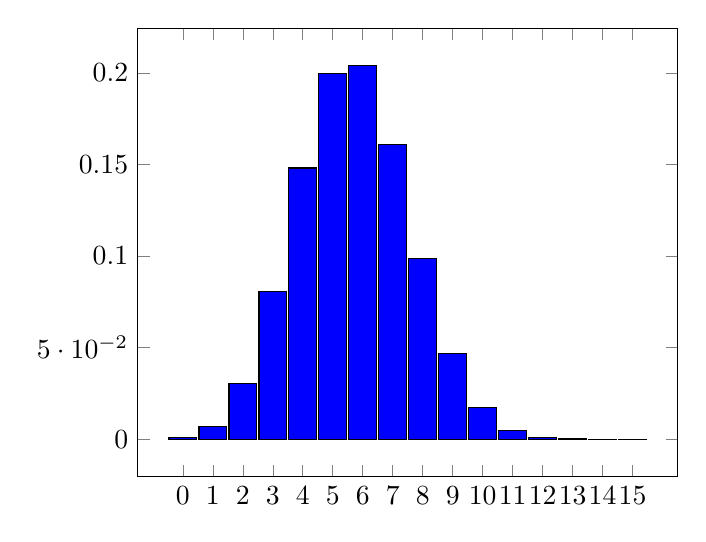
\begin{tikzpicture}
		\begin{axis}[
		symbolic x coords={$0$, $1$, $2$, $3$, $4$, $5$, $6$, $7$, $8$, $9$, $10$, $11$, $12$, $13$, $14$, $15$},
		xtick=data]
		\addplot[ybar,fill=blue] coordinates {
			($0$, 0.000768909705)
			($1$, 0.007069008578)
			($2$, 0.030328327124)
			($3$, 0.080549427953)
			($4$, 0.148107012687)
			($5$, 0.199705584849)
			($6$, 0.20400032861)
			($7$, 0.160756019319)
			($8$, 0.098527882808)
			($9$, 0.046968488937)
			($10$, 0.017272283029)
			($11$, 0.004811926357)
			($12$, 0.000983081729)
			($13$, 0.000139046299)
			($14$, 0.000012174561)
			($15$, 0.00000497455)
		};
		\end{axis}
		\end{tikzpicture}
	\subsubsection{Wahrscheinlichkeiten - y-Achse}
	Die y-Achse gibt die Wahrscheinlichkeit für das eintreten des Ereignisses der x-Achse an.
	
	\subsubsection{Ereignisse/Treffer - x-Achse}
	Die x-Achse gibt die Ereignisse bzw. die Anzahl der Treffer an.
	
	\subsubsection{Erwartungswert im Histogramm}
	Der Erwartungswert im Histogramm wird dadurch gekennzeichnet, dass er die höchste Säule besitzt. Er ist das Produkt aus der Wahrscheinlichkeit und n, also die Anzahl der Möglichkeiten.

	\subsubsection{Histogramme in Klausuren}
	Im Prüfungsteil A der Klausuren können Aufgaben drankommen wo man verschiedene Histogramme vor dem Hintergrund gegebener Kriterien bewerten soll. Bei solchen Aufgaben muss man meistens auf die 3 oben genannten Merkmale eines Histogramms achten. Entweder es gibt Wahrscheinlichkeiten für x-Werte die außerhalb des in der Aufgabenstellung definierten Bereiches liegen. \textbf{ODER} Die Summe aller Wahrscheinlichkeiten im Histogramm sind über 1. Dies ist bei korrekten Histogrammen keine Möglichkeit weshalb das Histogramm falsch ist und den in der Aufgabenstellung beschriebenen Kontext nicht darstellen. \textbf{ODER} Der Erwartungswert liegt nicht an der richtigen Stelle. \textbf{ODER} Eine Kombination von diesen drei Faktoren ist der Fall bzw. in verschiedenen Histogrammen vorhanden. Dies ist keine ausführliche Liste von Merkmalen die man bei Histogrammen analysieren kann, aber diese sind meistens die wichtigsten bei den Aufgaben in Klausuren.
\addcontentsline{toc}{section}{Bearbeitung einer Textaufgabe in der Klausur}
	\section*{Bearbeitung einer Textaufgabe in der Klausur}
	\begin{enumerate}
		\item $f(x) \ f^{\prime}(x) \ f^{\prime\prime}(x) \ f^{\prime\prime\prime}(x)$ hinschreiben und im CAS definieren
		\item Worfür steht x bzw. t, Wofür steht $f(x)$ bzw. $A(t)$ $\rightarrow$ Was bedeutet $f^{\prime}(x)$ bzw. $A^{\prime}(x)$
		\item Teilaufgaben genau lesen: Ist x \textbf{gegeben} oder \textbf{gesucht}? Ist f(x) \textbf{gegeben} oder \textbf{gesucht}?	
	\end{enumerate}

\end{document}